\chapter{Standards of Proof as Decision Rules}
\label{ch:standards}

\section{Two standards and one theory}

English law knows two standards of proof. In criminal cases the prosecution must make the jury sure of guilt, the modern form of proof beyond reasonable doubt. In civil cases the claimant must prove the facts on the balance of probabilities, which means that the fact is more probable than not. American law adds an intermediate standard, clear and convincing evidence, for matters such as fraud, civil commitment and the termination of parental rights. Civil law systems state their standards differently, as we shall see in Chapter~\ref{ch:commoncivil}, but they too distinguish criminal from civil proof.\index{standard of proof}

Decision theory explains these standards as thresholds on the posterior probability, each determined by the ratio of the losses from the two kinds of error. Equation \eqref{eq:threshold} gave the threshold, which we write here as $p^\ast = L_{FC}/(L_{FC} + L_{FA})$, where $L_{FC} = L(c,\bar G)$ is the loss from a false conviction, or more generally a false finding for the party bearing the burden, and $L_{FA} = L(a,G)$ the loss from a false acquittal. John Kaplan set out this analysis in 1968, and it has been refined many times since \citep{kaplan1968,kaye1999}. The civil standard corresponds to equal losses, $p^\ast = 1/2$. The criminal standard corresponds to a ratio of losses of perhaps ten or twenty to one, $p^\ast$ between about $0.9$ and $0.95$. The intermediate standard corresponds to an intermediate ratio.

The theory is simple. Its consequences are not. This chapter works through them: what the threshold implies about the meaning of reasonable doubt, how it interacts with the seriousness of the allegation, what it says about naked statistical evidence, and how Lindley used it to argue for graduated sanctions.

\section{What judges think reasonable doubt means}

Courts have generally refused to quantify reasonable doubt, and juries are told not to think in percentages. Yet when judges have been asked to translate the standard into a probability, their answers cluster. In \emph{United States v Fatico}, Judge Jack Weinstein reported an informal survey of his colleagues in the Eastern District of New York: their numerical equivalents for proof beyond reasonable doubt ranged from about three quarters to about ninety five per cent, with most near the upper end, and those for clear and convincing evidence clustered between about sixty and seventy five per cent \citep{fatico1978}. Surveys of jurors and students find wider dispersion and, worryingly, some respondents who place the criminal standard below the civil one. The dispersion matters. If one jury convicts at $0.75$ and another at $0.95$, the implied ratio of losses varies from three to nineteen, which is a large difference in the value the system places on avoiding false convictions.\index{reasonable doubt}

There is a principled reason courts avoid numbers: a fact finder who is told that ninety per cent suffices may treat a case at ninety per cent as a conviction, while one told only to be sure may hold out for more. Numbers can act as anchors. But the absence of numbers does not remove the threshold; it makes it invisible and variable. A Bayesian analysis cannot tell a society what ratio of losses to adopt. It can tell a society what ratio its procedures are in fact implementing, and whether that ratio is consistent across courts.

\section{The value of a correct decision depends on the stakes}

The simple threshold treats losses as fixed. In fact they vary with the seriousness of the charge, the severity of the sentence and the collateral consequences of conviction. A false conviction for murder is worse than a false conviction for shoplifting; so is a false acquittal. The threshold depends on their ratio, which need not change in any particular direction as seriousness increases. Some scholars argue, without agreement, that the criminal standard should rise with the sentence; others that it should fall for the gravest crimes, where the harm of a false acquittal is large. English law takes neither view for criminal cases: the standard is the same for all offences.\index{seriousness of allegation}

For civil cases the English courts went through a period of confusion. In \emph{Re H (Minors)} Lord Nicholls said that the more serious the allegation, the less likely it is that the event occurred, and hence the stronger the evidence needed before the court concludes that it is established on the balance of probabilities \citep{reh1996}. Lower courts read this as raising the standard for serious allegations. In \emph{Re B (Children)} the House of Lords corrected the reading: there is one civil standard, the balance of probabilities, and the seriousness of an allegation is relevant only so far as it bears on the inherent probability of the event \citep{reb2008}.

The Bayesian reading makes the distinction exact. Lord Nicholls was talking about the prior. Serious wrongdoing, such as the sexual abuse of a child or a fraud on a large scale, is usually rarer than minor wrongdoing, so its prior probability is lower, and more evidence is required to bring the posterior above one half. That is not a change in the threshold; it is a change in the starting point. Lady Hale in \emph{Re B} added that there is no necessary connection between seriousness and improbability, and Lord Hoffmann gave the example: if a child has been injured by one of only two people, it makes no sense to reason that injuring a child is serious and so neither is likely to have done it, since one of them did. The posterior threshold remains one half, and the prior is what it is. This is close to the Bayesian theory of the civil standard.

\section{Burden and prior}

The burden of proof says which party loses if the evidence leaves the fact finder at the threshold or below it. In decision terms it assigns the default action. The presumption of innocence is the criminal burden, but it has often been read as something stronger, a requirement that the fact finder begin with a prior probability of guilt of zero, or at least a small one. As we noted in Chapter~\ref{ch:why}, a prior of zero cannot be updated. The best Bayesian reading is that the defendant should be treated, before evidence specific to him is considered, as an exchangeable member of the population of people who could have committed the crime. If that population has $N$ members, his prior probability of guilt is $1/N$. Philip Dawid and others have defended this reading \citep{dawid2002}.\index{presumption of innocence}

The $1/N$ prior has attractive features. It does not depend on the fact that the defendant has been charged, which would be circular, since the charge reflects the evidence. It treats the defendant as an ordinary person. And it makes the role of evidence transparent: a conviction requires evidence whose combined Bayes factor exceeds roughly $N \cdot p^\ast/(1-p^\ast)$. For a crime that anyone in a city of a million could have committed and a threshold of $0.95$, this is about nineteen million, or seventy three decibans. A single DNA match with a random match probability of one in a billion and no error supplies ninety decibans and would suffice; on some estimates a single eyewitness supplies perhaps ten. Most convictions rest on many items of moderate weight that together cross the threshold.

\section{The gatecrasher and the expected utility solution}

Jonathan Cohen posed the gatecrasher problem in 1977 \citep{cohen1977}. At a rodeo 499 people pay for admission but 1{,}000 are counted in the seats; no tickets are issued, so nobody can show whether a given person paid. The organiser sues a randomly chosen attendee for the price of admission. With no other evidence, the probability that this person gatecrashed is $501/1000$, just over one half. On the balance of probabilities the organiser should win, and could win against every attendee, recovering $1{,}000$ admission fees when only $501$ are owed. Cohen used the example to argue that legal proof is not governed by the mathematical calculus of probability, and proposed an inductive, Baconian probability in its place.\index{gatecrasher paradox}

Several responses have been offered. One is that the probability is not really $0.501$, because, if tickets were issued (which departs from Cohen's stipulation), a ticket holder would usually keep the stub, and the defendant's failure to produce one is evidence. Another is that liability on naked statistics creates bad incentives, as in the blue bus case (Chapter~\ref{ch:odds}). Lindley took up the problem in his 1991 paper and offered a new solution within decision analysis \citep{lindley1991}. The solution we find most persuasive, in the spirit of that paper, starts from the observation that the paradox arises from forcing the court into an all or nothing choice. If the court could award damages equal to the probability of liability times the loss, it would award each attendee $0.501$ of the admission price, and the organiser would recover in total $501$ admission fees, exactly what it was owed. The expected utility solution reproduces the correct aggregate result, though not individual justice, since each of the 499 who paid is still charged $0.501$ of the fee. The paradox is a symptom of the binary system, not of probability.

The point generalises. Whenever the law insists on all or nothing remedies, it creates discontinuities at the threshold, and those discontinuities generate both injustice in individual cases and perverse incentives in the aggregate. Proportional remedies smooth the discontinuity (Figure~\ref{fig:losschance}). English law has accepted proportional damages in some contexts, notably loss of a chance in contract and professional negligence cases such as \emph{Allied Maples v Simmons and Simmons}, and refused it in others, notably in clinical negligence in \emph{Gregg v Scott} \citep{alliedmaples1995,gregg2005}. Chapter~\ref{ch:tort} examines these cases in detail.

\begin{figure}[t]
\centering
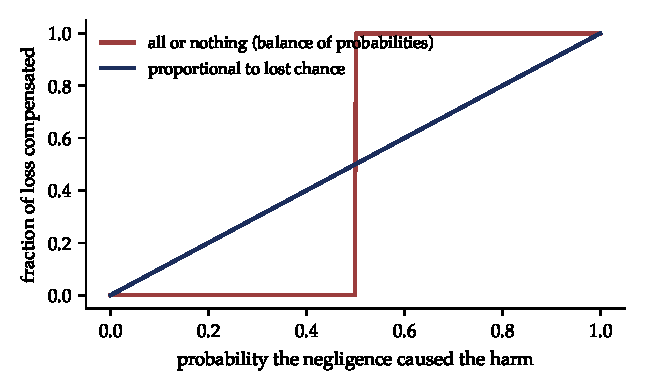
\includegraphics[width=\linewidth]{fig_loss_chance}
\caption{Compensation as a function of the probability that the defendant's breach caused the loss, under the all or nothing rule of the balance of probabilities and under proportional liability. The first has a jump at one half; the second is continuous.}
\label{fig:losschance}
\end{figure}

\section{Graduated sanctions}

Lindley also applied expected utility to criminal sentencing. Suppose the court can choose among acquittal, a light sentence and a heavy sentence, and suppose the losses are as in Table~\ref{tab:sanctions}. A light sentence imposed on an innocent person is a harm, but a smaller harm than a heavy one; a light sentence imposed on a guilty person is an under punishment, but less of a loss than an acquittal. Then for a middle range of posterior probabilities the light sentence minimises expected loss. In particular, there may be a range of probabilities below the conventional threshold for which some sanction is optimal \citep{lindley1991}.

\begin{table}[t]
\centering
\small
\begin{tabular}{lcc}
\toprule
Action & Loss if innocent & Loss if guilty\\
\midrule
Acquit & 0 & 10\\
Light sanction & 20 & 4\\
Heavy sanction & 100 & 0\\
\bottomrule
\end{tabular}
\caption{An illustrative loss table for three actions. Expected losses are $10p$, $20(1-p) + 4p$ and $100(1-p)$. Acquittal is optimal for $p < 0.77$, the light sanction for $0.77 < p < 0.95$, and the heavy sanction above.}
\label{tab:sanctions}
\end{table}

This conclusion is uncomfortable, and Lindley knew it. It conflicts with the principle that no one should be punished unless proved guilty, a principle that is constitutive of the criminal law rather than an instrumental rule. The Bayesian can respond that the principle is itself a statement about utilities: society may attach a large disutility to any punishment of a person not proved guilty, beyond the direct harm of the punishment, because such punishment undermines trust in law. If that disutility is large enough (in Table~\ref{tab:sanctions}, at least $100$), the light sanction disappears from the optimal set altogether. The framework accommodates the principle; it asks that its cost be made explicit. In practice the criminal law has many graduated responses that operate below the full criminal standard: bail conditions, protective orders, civil recovery, and regulatory sanctions. The decision theoretic view helps organise these and ask whether their thresholds are consistent.

\section{The value of information and when to stop}

A court does not only decide; it decides when to decide. Adjournments, further disclosure, expert reports and retrials all buy information at a cost. The expected value of sample information is the reduction in expected loss from the decision that the new information makes possible, before the information is seen. If the posterior is already far from the threshold, new evidence is unlikely to change the decision and is worth little. If the posterior is near the threshold, even modest evidence may tip it, and its value is high.\index{value of information}

Formally, let the current posterior be $p$ and suppose a further item of evidence would have Bayes factor $B$ with known distribution under each hypothesis. The value of obtaining it is
\begin{equation}
\mathrm{VOI}(p) = \min\{p L_{FA}, (1-p)L_{FC}\} - \E\left[\min\{p' L_{FA}, (1-p') L_{FC}\}\right],
\end{equation}
where $p'$ is the updated posterior and the expectation is taken under the current predictive distribution. This is always non negative and is largest near $p^\ast$. A court acting rationally would buy information when $\mathrm{VOI}(p)$ exceeds its cost, which includes delay. Chapter~\ref{ch:india} applies this idea to triage in an overloaded court system, where the cost of delay is high and the court must decide which cases to hear first.

\section{Multiple elements and the conjunction problem}

A claim usually has several elements, each of which must be proved. In negligence the claimant must prove duty, breach, causation and damage. If each element is proved to probability $0.7$ and they are independent, is the claim proved? Each element is more probable than not, but their conjunction has probability $0.7^4 \approx 0.24$. This is the conjunction paradox, another of Cohen's challenges \citep{cohen1977}.\index{conjunction paradox}

Courts in fact apply the standard element by element, and there are good reasons for this. The elements are rarely independent: evidence that the defendant drove carelessly also makes it more probable that the carelessness caused the collision. Even so, the decision theoretic threshold applies to the decision, and the decision whether the defendant is liable depends on the probability that all elements hold. A court that finds each element at $0.7$ and gives judgment for the claimant is, on a strict Bayesian view, deciding wrongly unless the elements are highly correlated. Legal scholars have proposed various resolutions, including Michael Pardo and Ronald Allen's view that the fact finder should infer the best explanation rather than apply a probability threshold, and Allen's relative plausibility theory, in which the fact finder compares the parties' stories \citep{allen2019}. We think the story based theories are best understood as Bayesian model comparison, which is the subject of Chapter~\ref{ch:stories}.

\section{Scotland's third verdict}

Scotland long allowed three verdicts in criminal trials: guilty, not guilty and not proven. Not proven had the same legal effect as not guilty but was widely understood to mean that the jury suspected guilt without being sure. Critics argued that it stigmatised acquitted defendants and confused juries, and the Scottish Parliament has abolished it, for trials beginning on or after 1 January 2026 (Victims, Witnesses, and Justice Reform (Scotland) Act 2025). In decision theoretic terms the third verdict did not create a third action, since its consequences were those of acquittal, but it communicated information about the posterior. It told the public that the jury's posterior lay in a middle band. A Bayesian could argue for keeping it as a signal while recognising that its legal effect was nil. The debate about it was a debate about whether courts should publish their posteriors, a question that will become more pressing when machines produce probabilities as a matter of course.

\section{Summary}

Standards of proof are decision thresholds. The civil standard is the threshold for equal losses; the criminal standard reflects a judgment that false convictions are much worse than false acquittals. In English civil law, the seriousness of an allegation affects the prior, not the threshold. Naked statistical evidence is problematic because of incentives and because of the binary system, not because probability is irrelevant. A proportional remedy, the expected utility solution, removes the aggregate overrecovery in the gatecrasher paradox and has analogues in the law of loss of a chance. And the value of information tells a court when it should seek more evidence before deciding.

\section*{Notes and Questions}
\addcontentsline{toc}{section}{Notes and Questions}
\begin{enumerate}[label=\arabic*.]
\item Find the ratio of losses implied by thresholds of $0.75$, $0.9$ and $0.95$. If juries in different courts apply these thresholds, how much does the implied value of avoiding a false conviction vary?
\item In the gatecrasher problem, suppose ticket holders keep their stubs with probability $0.8$ and the defendant cannot produce one. Compute the posterior probability that he gatecrashed.
\item Using Table~\ref{tab:sanctions}, find the expected loss of each action at $p = 0.8$. Add a disutility of $50$ to any sanction imposed on an innocent person and redo the analysis.
\item Show that the value of information is zero when the posterior is zero or one and is maximised at or near the threshold.
\item Suppose duty, breach, causation and damage are each proved to $0.8$ and are equally and positively correlated (a common pairwise correlation), with a joint distribution of your choice. What is the probability that all four hold? What common correlation would make it exceed one half?
\item Read the speeches in \emph{Re B (Children)}. Identify every passage that can be read as a statement about priors, likelihoods or thresholds.
\end{enumerate}

\section*{Further reading}
Kaplan's 1968 article is the starting point \citep{kaplan1968}. Kaye surveys Bayesian decision rules for the burden of persuasion \citep{kaye1999}. Lindley's 1991 paper should be read in full \citep{lindley1991}. Cohen's \emph{The Probable and the Provable} is the classic statement of the opposing view \citep{cohen1977}.
